%%%%%%%%%%%%%%%%%%%%%%%%%%%%%%%%%%%%%%%%%
% Uppsala University Assignment Title Page 
% LaTeX Template
% Version 1.0 (27/12/12)
%
% This template has been downloaded from:
% http://www.LaTeXTemplates.com
%
% Original author:
% WikiBooks (http://en.wikibooks.org/wiki/LaTeX/Title_Creation)
% Modified by Elsa Slattegard to fit Uppsala university
% License:
% CC BY-NC-SA 3.0 (http://creativecommons.org/licenses/by-nc-sa/3.0/)

%\title{Title page with logo}
%----------------------------------------------------------------------------------------
%	PACKAGES AND OTHER DOCUMENT CONFIGURATIONS
%----------------------------------------------------------------------------------------

\documentclass[12pt]{article}

\usepackage{tikz,lipsum,lmodern}
\usepackage[most]{tcolorbox}

\usepackage[utf8]{inputenc}
\usepackage[greek,english]{babel}
\usepackage{alphabeta}
\usepackage{amsmath}
\usepackage{gfsartemisia}
\usepackage{graphicx}
\usepackage{subfig}
\usepackage{float}
\usepackage[colorinlistoftodos]{todonotes}
\usepackage{tabularx}
\usepackage[myheadings]{fullpage}
\usepackage{enumitem}
\PassOptionsToPackage{hyphens}{url}\usepackage{hyperref}
\usepackage{tikz}
\usepackage[nottoc]{tocbibind} %Adds "References" to the table of contents
\usepackage{xcolor} % to access the named colour LightGray
\definecolor{LightGray}{gray}{0.9}

\usepackage[edges]{forest}
\definecolor{folderbg}{RGB}{124,166,198}
\definecolor{folderborder}{RGB}{110,144,169}

%================ file tree =====================%
\usepackage[edges]{forest}
\definecolor{folderbg}{RGB}{124,166,198}
\definecolor{folderborder}{RGB}{110,144,169}
\newlength\Size
\setlength\Size{4pt}
\tikzset{%
	folder/.pic={%
		\filldraw [draw=folderborder, top color=folderbg!50, bottom color=folderbg] (-1.05*\Size,0.2\Size+5pt) rectangle ++(.75*\Size,-0.2\Size-5pt);
		\filldraw [draw=folderborder, top color=folderbg!50, bottom color=folderbg] (-1.15*\Size,-\Size) rectangle (1.15*\Size,\Size);
	},
	file/.pic={%
		\filldraw [draw=folderborder, top color=folderbg!5, bottom color=folderbg!10] (-\Size,.4*\Size+5pt) coordinate (a) |- (\Size,-1.2*\Size) coordinate (b) -- ++(0,1.6*\Size) coordinate (c) -- ++(-5pt,5pt) coordinate (d) -- cycle (d) |- (c) ;
	},
}
\forestset{%
	declare autowrapped toks={pic me}{},
	pic dir tree/.style={%
		for tree={%
			folder,
			font=\ttfamily,
			grow'=0,
		},
		before typesetting nodes={%
			for tree={%
				edge label+/.option={pic me},
			},
		},
	},
	pic me set/.code n args=2{%
		\forestset{%
			#1/.style={%
				inner xsep=2\Size,
				pic me={pic {#2}},
			}
		}
	},
	pic me set={directory}{folder},
	pic me set={file}{file},
}

%=================================================%


\usepackage{tabto}
\usepackage{minted}


\hyphenpenalty=10000


\usepackage{geometry}
\geometry{
	a4paper,
	total={170mm,257mm},
	left=20mm,
	top=20mm,
}


\addto\captionsenglish{% Replace "english" with the language you use
	\renewcommand{\contentsname}%
	{Περιεχόμενα}%
}

\addto\captionsenglish{
	\renewcommand{\partname}{}
}
\renewcommand{\thepart}{}

\makeatletter
\renewcommand{\fnum@figure}{Εικόνα \thefigure}
\makeatother


\renewcommand{\H}{\textlozenge}

%=====fonts==========%
%\usepackage{libertine}


%====================%





%=============header + footer ======================%
%

\usepackage{fancyhdr}

\pagestyle{fancy}
\fancyhf{}
\rhead{Σύγχρονα θέματα Τεχνολογίας Λογισμικού 
\includegraphics[width=0.7cm]{UNIPI_(logo).png}}
\lhead{Πανεπιστήμιο Πειραιώς \\ Τμήμα Πληροφορικής}
\cfoot{Σελίδα \thepage}

% 

%\setlength\headheight{47pt}
%=====================================================%



%\setcounter{secnumdepth}{0} % sections are level 1

\begin{document}
	
	\begin{titlepage}
		
		\newcommand{\HRule}{\rule{\linewidth}{0.5mm}} % Defines a new command for the horizontal lines, change thickness here
		
		\center % Center everything on the page
		
		%----------------------------------------------------------------------------------------
		%	HEADING SECTIONS
		%----------------------------------------------------------------------------------------
		
		\textsc{\LARGE Πανεπιστήμιο Πειραιώς}\\[1.5cm] % Name of your university/college
		
\includegraphics[scale=0.6]{UNIPI_(logo).png}\\[1cm] % Include a department/university logo - this will require the graphicx package
		\textsc{\Large Τμήμα Πληροφορικής}\\[0.5cm] % Major heading such as course name
		\textsc{\large Σύγχρονα θέματα Τεχνολογίας Λογισμικού - Λογισμικό για κινητές συσκευές}\\[0.5cm] % Minor heading such as course title
		
		%----------------------------------------------------------------------------------------
		%	TITLE SECTION
		%----------------------------------------------------------------------------------------
		
		\HRule \\[0.4cm]
		{ \Large \bfseries Αριστοτέλης Ματακιάς - Α.Μ: Π19100}\\[0.4cm] % Title of your document
		{ \Large \bfseries Βασίλη Γκιάτα - Α.Μ. Π19036}\\[0.4cm] % Title of your document
		\HRule \\[1.5cm]
		
		%----------------------------------------------------------------------------------------
		%	AUTHOR SECTION
		%----------------------------------------------------------------------------------------
		%
		
		\textsc{\Large Εργασία στο μοντέλο Model View Controller \\[0.4cm] Τεχνικό Εγχειρίδιο} % Minor heading such as course title
		
		% If you don't want a supervisor, uncomment the two lines below and remove the section above
		%\Large \emph{Author:}\\
		%John \textsc{Smith}\\[3cm] % Your name
		
		%----------------------------------------------------------------------------------------
		%	DATE SECTION
		%----------------------------------------------------------------------------------------
		
		
		
		\vfill % Fill the rest of the page with whitespace
		
	\end{titlepage}
	
	%\selectlanguage{greek}
	\tableofcontents
	%\selectlanguage{english}
	
	 \newpage
	
%	 \section{Εισαγωγή}
%	 Στο παρόν έγγραφο περιλαμβάνεται η τεχνική αναφορά για το project με τίτλο \textbf{UniveristyApp} (ASP.NET Core Web Application). Η γλώσσα προγραμματισμού είναι C\# και η βάση δεδομένων δημιουργήθηκε με το εργαλείο Microsoft Sql Server 2022.
%	 
%	 Στις ενότητες που ακολουθούν αναλύονται αρχικά τα ζητούμενα της εργασίες και στην συνέχεια οι λεπτομέρειες υλοποίησης όπου αναλύονται τα επίπεδα \textbf{Model}, \textbf{View} και \textbf{Controller}.
%	
%	 \newpage
	
	\section{Ζητούμενα}
	
	Να αναπτύξετε μια διαδικτυακή εφαρμογή βαθμολογίου για τους φοιτητές του πανεπιστημίου. Η εφαρμογή θα περιλαμβάνει διάφορες κατηγορίες χρηστών όπως \textbf{φοιτητές}, \textbf{καθηγητές} και \textbf{γραμματειακό προσωπικό}. Για παράδειγμα, ένας καθηγητής μπορεί να καταχωρήσει τη βαθμολογία για κάθε φοιτητή και για κάθε μάθημα που διδάσκει (τελικό βαθμό ή/και επιμέρους βαθμούς του μαθήματος όπως βαθμοί από ασκήσεις, εργασίες, γραπτό διαγώνισμα), ενώ κάθε φοιτητής μπορεί να έχει πρόσβαση στο λογαριασμό του ώστε να δει τα αποτελέσματα της βαθμολογίας του.
		
	Όλοι οι Χρήστες θα μπορούν να κάνουν Login μέσω μιας Φόρμας Login (η επιτυχής σύνδεση θα ανακατευθύνει τον χρήστη στην index σελίδα).
	
	\begin{itemize}
		
		\item Για τους Φοιτητές:
		\begin{itemize}
			\item[$\blacksquare$] Προβολή βαθμολογίας ανά μάθημα.
			\item[$\blacksquare$] Προβολή βαθμολογίας ανά εξάμηνο.
			\item[$\blacksquare$] Προβολή συνολικής βαθμολογίας (για όλα τα μαθήματα που έχει εξεταστεί).
		\end{itemize}
	
		\item Για τους Καθηγητές:
		\begin{itemize}
			\item[$\blacksquare$] Προβολή λίστας βαθμολογίας ανά μάθημα (για ήδη βαθμολογημένα μαθήματα).
			\item[$\blacksquare$] Καταχώρηση βαθμολογίας ανά μάθημα (για μη βαθμολογημένα μαθήματα).
		\end{itemize}
	
		\item Για τις Γραμματείες:
		\begin{itemize}
			\item[$\blacksquare$] Καταχώρηση Μαθημάτων, Καθηγητών, Φοιτητών.
			\item[$\blacksquare$] Προβολή μαθημάτων (τίτλος μαθήματος, εξάμηνο, υπεύθυνος Καθηγητής).
			\item[$\blacksquare$] Ανάθεση μαθήματος σε Καθηγητή.
			\item[$\blacksquare$] Δήλωση μαθήματος σε Φοιτητή.
		\end{itemize}
	
	\end{itemize}
	
	\newpage
	\section{Επίπεδο Model}
	Η υλοποίηση της εφαρμογής ξεκίνησε αρχικά από την δημιουργία της βάσης δεδομένων. Παρακάτω δίνεται το σχεσιακό σχήμα της βάσης.
	
	\begin{figure}[H]
		\centering
		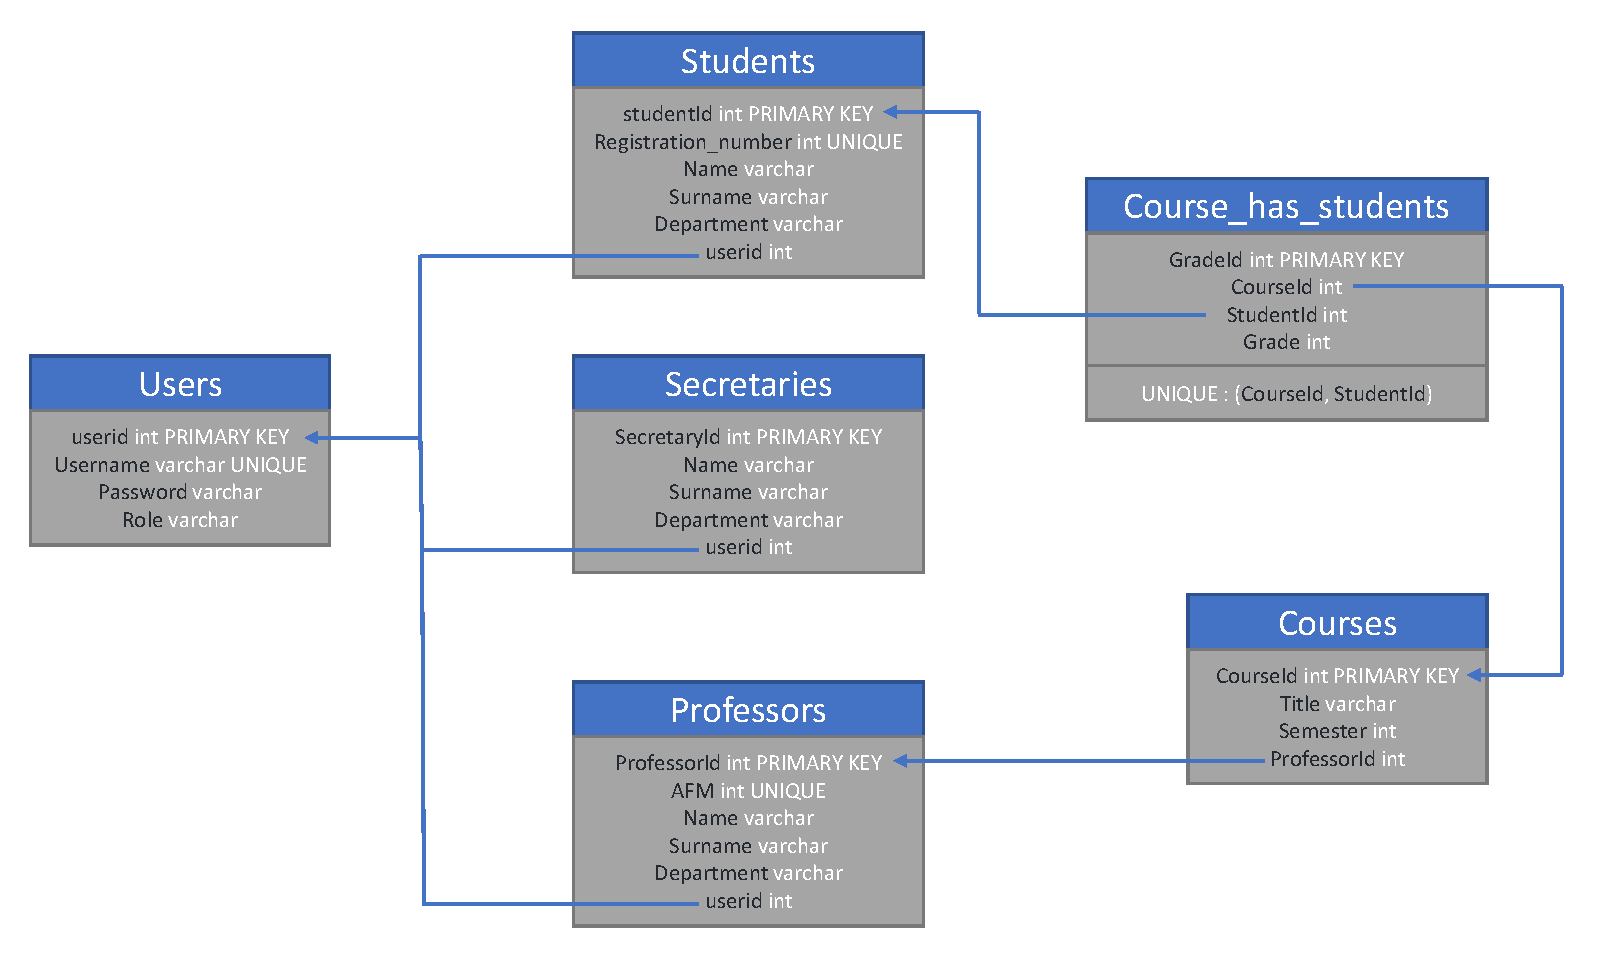
\includegraphics[width=0.85\textwidth]{table.pdf}
		\caption{}
		\label{fig:bex}
	\end{figure}
	
	Αρχικά υπάρχει ο πίνακας \textbf{Users} στον οποίο περιλαμβάνονται οι κωδικοί πρόσβασης (username και password) όλων των χρηστών της εφαρμογής. Το πεδίο UserID είναι απλώς ένας κωδικός ξεχωριστός για κάθε χρήστη και το πεδίο Role δηλώνει τον τύπο του χρήστη. Στην εφαρμογή υπάρχουν 3 βασικοί τύποι χρηστών: \textbf{Students (Φοιτητές)}, \textbf{Professors (Καθηγητές)} και \textbf{Secretaries (Γραμματείες)}. Υπάρχουν οι 3 αντίστοιχοι πίνακες οι οποίοι συνδέονται με τον πίνακα \textbf{Users} μέσω του ξένου κλειδιού (foreign key) UserID. Ο πίνακας Users θα μπορούσε να παραληφθεί αλλά επιτρέπει την εύκολη υλοποίηση του \textbf{Session Management} που θα αναλυθεί σε επόμενη ενότητα.
	
	Στη συνέχεια υπάρχει ο πίνακας \textbf{Courses} όπως δηλώνει το όνομά του περιέχει τα Μαθήματα. Κάθε μάθημα ανατίθεται σε έναν καθηγητή αποκλειστικά, γι' αυτό υπάρχει το πεδίο ProfessorId το οποίο είναι foreign key και δείχνει στο PK του πίνακα \textbf{Professors}.
	
	Ο πίνακας \textbf{Course\_has\_students} συνδέει τις εγγραφές των πινάκων \textbf{Students} και \textbf{Courses}. Περιέχει τα πεδία StudentId και CourseId τα οποία είναι foreign keys και στα PK των πινάκων \textbf{Students} και \textbf{Courses} αντίστοιχα. Επιπλέον ορίζεται ως unique το ζευγάρι των πεδίων StudentId και CourseId. Αυτό γίνεται διότι μπορεί ένας φοιτητής να έχει πολλές εγγραφές στον πίνακα \textbf{Course\_has\_students}, άρα το StudentId θα επαναλαμβάνεται, και αντίστοιχα πολλοί φοιτητές θα έχουν το ίδιο μάθημα άρα το CourseId θα επαναλαμβάνεται. Δεν πρόκειται όμως στον πίνακα \textbf{Course\_has\_students} να εισαχθεί ο ίδιος φοιτητής με το ίδιο μάθημα πάνω από μία φορά, γι' αυτό ορίζεται ο αντίστοιχος περιορισμός 2 πεδίων.
	
	Σε όλους τους πίνακες έχει οριστεί ένα Id σαν PK. Αυτό έγινε καθώς το scaffolding του Visual Studio 2022 αναγνωρίζει καλύτερα τις σχέσεις μεταξύ των πινάκων. Θεωρούμε πως σε κάθε πίνακα το Id είναι ένας αύξοντας αριθμός (AUTO INCREMENT). Οι κλάσεις των μοντέλων που προέκυψαν περιέχονται στον φάκελο Models ο οποίος έχει την παρακάτω αρχειοθέτηση:
	
\begin{figure}[H]
	\centering
	\begin{forest}
		pic dir tree,
		where level=0{}{% folder icons by default; override using file for file icons
			directory,
		},
		[Models
		[Metadata
		[CourseMetadata.cs, file
		]
		[ProfessorMetadata.cs, file
		]
		[StudentMetadata.cs, file
		]
		]
		[Course.cs, file
		]
		[CourseHasStudent.cs, file
		]
		[ErrorViewModel.cs, file
		]
		[PatialClasses.cs, file
		]
		[Professor.cs, file
		]		
		[Secretary.cs, file
		]
		[Student.cs, file
		]
		[UniveristyDBContext.cs, file
		]
		[User.cs, file
		]	
		]
	\end{forest}
	\caption{Αρχειοθέτηση του φακέλου Models}
\end{figure}
	
	Έχουν προστεθεί και Metadata κλάσεις κυρίως για την αλλαγή DisplayNames πεδίων και τη δημιουργεία computed πεδίων (όπως Fullname).
		
	\section{Επίπεδο View και Controller}
	
	\subsection{Session Management}
	Στην εκφώνηση της εργασίας αναφέρεται ότι η υλοποίηση Session Management δεν περιλαμβάνεται στα ζητούμενα. Ωστόσο αποφασίστηκε στα πλαίσια της εργασίας να συμπεριληφθεί η διαχείριση Συνόδου μέσω μίας απλής υλοποίησης. Πιο συγκεκριμένα δεν χρησιμοποιήθηκε το Microsoft Identity Platform που παρέχεται από το Visual Studio 2022 αλλά ένα custom Session management μέσω μεθόδων που περιέχονται ήδη στο MVC project.
	
	Για να γίνει πιο κατανοητή η διαδικασία θα ξεκινήσουμε με ένα παράδειγμα. Παρακάτω δίνεται μια C\# εντολή στην οποία δημιουργείται στο session ένα πεδίο string με όνομα username και περιεχόμενο 'user1'

\begin{minted}
[
frame=lines,
framesep=2mm,
baselinestretch=1.2,
bgcolor=LightGray,
fontsize=\footnotesize
]{csh}
HttpContext.Session.SetString("username", "user1");
\end{minted}

Εφόσον η εντολή αυτή εκτελεστεί, μπορούμε στη συνέχεια να ανακτήσουμε το περιεχόμενο του πεδίου username από το session με την παρακάτω εντολή:

\begin{minted}
[
frame=lines,
framesep=2mm,
baselinestretch=1.2,
bgcolor=LightGray,
fontsize=\footnotesize
]{csh}
HttpContext.Session.GetString("username")
\end{minted}

Η εντολή αυτή επιστρέφει ένα string και είναι το περιεχόμενο του πεδίου username. Πάνω σε αυτές τις εντολές βασίζεται η διαχείριση συνόδου της εφαρμογής.

Η είσοδος του χρήστη πραγματοποιείται μέσω του View \textbf{Login.cshmtl} το οποίο είναι προσβάσιμο από την αρχική σελίδα (index) του HomeController (ο οποίς είναι και ο default controller). Σε αυτό το View ο χρήστης δίνει το Username και το Password του και εκτελείται η παρακάτω Action Method.

\begin{minted}
	[
	frame=lines,
	framesep=2mm,
	baselinestretch=1.2,
	bgcolor=LightGray,
	fontsize=\footnotesize
	]{csh}
[HttpPost]
public ActionResult Login(User user)
{
	_context = new UniversityDBContext();
	var obj = _context.Users.Where(a => a.Username.Equals(user.Username) 
		&& a.Password.Equals(user.Password)).FirstOrDefault();
	if (obj != null)
	{
		HttpContext.Session.SetString("username", obj.Username.ToString());
		HttpContext.Session.SetString("userid", obj.Userid.ToString());
		HttpContext.Session.SetString("role",obj.Role.ToString());
		
		return RedirectToAction("Index", obj.Role);
	}	
	return RedirectToAction("Login");
}
\end{minted}
Μέσω ενός Post request στέλνεται στον Server ένα αντικείμενο τύπου User (περιέχει μόνο τα πεδία Username και Password - τα υπόλοιπα είναι \textbf{null}) και γίνεται έλεγχος αν υπάρχει στην βάση User με τα δοσμένα credentials. Αν δεν βρεθεί χρήστης, γίνεται Redirection στην Log in σελίδα. Αντίθετα, αν βρεθεί το αντίστοιχο User object, δημιουργούνται 3 πεδία στο Session:

\begin{itemize}
	\item Πεδίο \textbf{username} το οποίο περιέχει το Username του αντικειμένου User
	\item Πεδίο \textbf{userid} το οποίο περιέχει το UserId του αντικειμένου User
	\item Πεδίο \textbf{role} το οποίο περιέχει το Role του αντικειμένου User
\end{itemize} 

Οι πληροφορίες αυτών των πεδίων είναι απαραίτητες, καθώς χάρις αυτές θα καθορίζεται σε ποιες λειτουργίες της εφαρμογής θα έχει πρόσβαση ο χρήστης που συνδέθηκε. Για παράδειγμα ένας Καθηγητής μπορεί να δει μόνο τα δικά του μαθήματα και τις αντίστοιχες βαθμολογίες του και όχι μαθήματα άλλων καθηγητών. Αντίστοιχα δεν επιτρέπεται ένας Φοιτητής ή ένας Καθηγητής να έχει πρόσβαση σε σελίδες της Γραμματείας. Πριν εξηγήσουμε πώς θα γίνονται αυτοί οι έλεγχοι πρέπει να αναφέρουμε την γενική δομή των Controller της εφαρμογής. Όπως φαίνεται στην παραπάνω συνάρτηση \textbf{Login} μετά τον ορισμό των πεδίων του Session ο χρήστης ανακατευθύνεται στην Index σελίδα του controller με όνομα το περιεχόμενο του πεδίου \textbf{user.Role}. Από σύμβαση της Βάσης Δεδομένων Users που είναι οι Φοιτητές, οι Καθηγητές και οι Γραμματείες περιέχουν στο πεδίο Role την λέξη 'Students', 'Professors' και 'Secretaries' αντίστοιχα. Οι τρεις αυτοί όροι αντιστοιχοούν στους Controllers της εφαρμογής: \textbf{StudentsController}, \textbf{ProfessorsController} και \textbf{SecretariesController}.

Κάθε ένας Controller περιέχει όλες τις λειτουργίες του τύπου χρήστη στον οποίο αντιστοιχούν. Δηλαδή όταν ένας Φοιτητής δώσει τους κωδικούς του, θα μεταβεί στην Index του StudentsController και όλες οι λειτουργίες και τα Views στα οποία θα έχει πρόσβαση περιέχονται στον παρόντα Controller. Το ίδιο ισχύει για τους Καθηγητές (ProfessorsController) και τους Γραμματείς (SecretariesController). Στη πράξη αυτό σημαίνει ότι ένας χρήστης \textbf{πρέπει} να έχει πρόσβαση μόνο στις μεθόδους του Controller που του αντιστοιχεί. Ο έλεγχος αυτός αποτελείται από δύο μέρη:

\begin{enumerate}
	\item Ελέγχεται αν ο χρήστης δεν είναι συνδεδεμένος και προσπαθεί να μεταβεί σε μια σελίδα που χρειάζονται credentials και
	
	\item Ελέγχεται αν ο χρήστης που έχει συνδεθεί επιτυχώς προσπαθεί να μεταβεί σε μια σελίδα που δεν έχει δικαίωμα να δει.
\end{enumerate}

Στην πρώτη περίπτωση ελέγχεται αν το userId του session είναι null, ενώ στη δεύτερη περίπτωση ελέγχεται αν το role του session είναι το ίδιο με το role του χρήστη (αντικείμενο User) που είναι συνδεδεμένος. Και στις δυο περιπτώσεις αν ο έλεγχος αποτύχει, η Action Method ανακατευθύνει τον χρήστη σε αντίστοιχο View και η εκτέλεση σταματάει. Παρακάτω δίνεται ένα παράδειγμα μίας μεθόδου του StudentsController.

\begin{minted}
	[
	frame=lines,
	framesep=2mm,
	baselinestretch=1.2,
	bgcolor=LightGray,
	fontsize=\footnotesize
	]{csh}
[ResponseCache(NoStore = true, Location = ResponseCacheLocation.None)]
public IActionResult Grades(string? sortOrder)
{
	if (HttpContext.Session.GetString("userid") == null)
		return View("AuthorizationError");
	
	if (!(HttpContext.Session.GetString("role").Equals("Students")))
		return View("NoRightsError");
	
	var student = StudentGetter();
	
	// rest of the code ...
\end{minted}

Πριν την εκτέλεση του Bisness Logic μιας Action Method τοποθετούνται δύο συνθήκες if οι οποίες αντιστοιχούν στους δύο ελέγχους που παρουσιάστηκαν: η πρώτη συνθήκη ελέγχει αν ο χρήστης έχει κάνει Log in και η δεύτερη συνθήκη ελέγχει αν ο ρόλους αποθηκευμένος στο session είναι σωστός, στη συγκεκριμένη περίπτωση επειδή αυτή η μέθοδος 'ανήκει' στις λειτουργίες του φοιτητή ο ρόλος πρέπει να περιέχει τη λέξη 'Students'. Και οι δύο συνθήκες όταν ενεργοποιηθούν ανακατευθύνουν τον χρήστη σε αντίστοιχα Views (AuthorizationError και NoRightsError). Τα Views αυτά περιέχονται στον φάκελο Views\textbackslash Shared ώστε να είναι προσβάσιμα από όλους τους Controller και περιέχουν αντίστοιχα μηνύματα ενημέρωσης για τον χρήστη.

% 2 εικονες side by side

Μια σημαντική λεπτομέρεια που δεν εξηγήθηκε στον κώδικα της προηγούμενης μεθόδου είναι ποιος είναι ο ρόλος του tag:

\begin{minted}
	[
	frame=lines,
	framesep=2mm,
	baselinestretch=1.2,
	bgcolor=LightGray,
	fontsize=\footnotesize
	]{csh}
[ResponseCache(NoStore = true, Location = ResponseCacheLocation.None)]
	\end{minted}
Το συγκεκριμένο tag τοποθετήθηκε στην μέθοδο ώστε το View που επιστρέφεται στον Browser να μην αποθηκεύεται στην cache. Έτσι αν το session λήξει ή ο χρήστης κάνει log out, δεν θα είναι προσβάσιμες οι σελίδες που φορτώθηκαν αν χρησιμοποιηθεί η εντολή "πίσω" του browser.

Τέλος, πρέπει να εξηγηθεί πώς ένας χρήστης μπορεί να αποσυνδεθεί (να κάνει log out) από τον λογαριασμό του όταν ολοκληρώσει τις ενέργειές του. Η λήξη της συνόδου από τον χρήστη γίνεται από την συνάρτηση Logout του HomeController.
\newpage
\begin{minted}
	[
	frame=lines,
	framesep=2mm,
	baselinestretch=1.2,
	bgcolor=LightGray,
	fontsize=\footnotesize
	]{csh}
public ActionResult Logout()
{
	HttpContext.Session.Clear();
	HttpContext.Session.Remove("username");
	HttpContext.Session.Remove("userid");
	HttpContext.Session.Remove("role");
	return RedirectToAction("Index");
}
\end{minted}

Όπως φαίνεται η συγκεκριμένη μέθοδος αφαιρεί όλα τα πεδία που εισάχθηκαν στο session κατά την είσοδο και ανακατευθύνει τον χρήστη στην αρχική σελίδα Home page.

\subsection{Layout Razor View}
Βασικό μέρος του presentation layer (ή αλλιώς View layer) είναι το \textbf{\_Layout.cshtml}. Το αρχείο αυτό περιλαμβάνεται στον φάκελο Shared και φορτώνεται μαζί με κάθε View Που εμφανίζεται στον browser. Στο αρχείο αυτό γίνεται import το css αρχείο του Bootstrap Framework. Πιο συγκεκριμένα δεν χρησιμοποιήθηκε το css αρχείο που ήδη περιλαμβάνεται στο Visual Studio, αλλά ένα Custom Themed Bootstrap css που δίνει πιο ιδανικά χρώματα σε όλη την εφαρμογή.

Επιπλέον στο \textbf{\_Layout.cshtml} περιλαμβάνεται η μπάρα περιήγησης ή αλλιώς navigation bar. Η συγκεκριμένη μπάρα έχει στα αριστερά 3 συνδέσμους: έναν για το Home page, έναν για το News και έναν για το About page. Οι σελίδες αυτές ανήκουν στον HomeController και θα αναλυθούν σε λίγο. Πιο μεγάλη βαρύτητα έχει ο σύνδεσμος του navbar που βρίσκεται στα δεξιά καθώς όπως φαίνεται στο κώδικα μέσω συνθηκών if αλλάζει ανάλογα με το αν ο χρήστης είναι ή όχι συνδεδεμένος.

% 4 images

Αν ο χρήστης δεν έχει συνδεθεί τότε ο σύνδεσμος απλά τον πάει στο Log in page. Αν όμως ο χρήστης έχει συνδεθεί, τότε ο σύνδεσμος αντικαθίσταται με ένα μενού επιλογών. Το μενού περιέχει όλες τις βασικές σελίδες που αντιστοιχούν στον συγκεκριμένο τύπο χρήστη καθώς και την επιλογή Log out. Ο τίτλος του μενού έχει το username του χρήστη.

Στο κάτω μέρος της σελίδας υπάρχει και ένας footer που περιέχει το όνομα της εφαρμογής και ένα λινκ για την σελίδα License.

\subsection{Home Controller}
Ο HomeController είναι υπεύθυνος για να φορτώνει τις "στατικές" σελίδες της εφαρμογής και αυτές είναι η Index, η News, η About, η Login και η License. Οι σελίδες αυτές αναφέρονται ως στατικές καθώς δεν δέχονται δεδομένα από την βάση δεδομένων της εφαρμογής.

Οι μέθοδοι του HomeController είναι αρκετά απλές με εξαίρεση την POST Login και την GET Logout οι οποίες έχουν ήδη αναλυθεί σε προηγούμενη ενότητα καθώς αφορούν το Session Management. Οι υπόλοιπες μέθοδοι απλά επιστρέφουν το αντίστοιχο View.

Σχετικά με τα Views του HomeController έχουν να επισημανθούν τα εξής:

\begin{itemize}
	
	\item \textbf{Index}:\\
	Αποτελεί την κεντρική σελίδα (Home page) της εφαρμογής. Σε αυτήν εμφανίζονται σύντομες και γενικές πληροφορίες για το Πανεπιστήμιο για το οποίο φτιάχτηκες η εφαρμογή. Στη συγκεκριμένη περίπτωση θεωρείται ότι το πανεπιστήμιο είναι το Πανεπιστήμιο Πειραιά. Η σελίδα αυτή βασίστηκε στο παράδειγμα Carousel της σελίδας Bootstrap.
	
	\item \textbf{News}:\\
	Σε αυτή τη σελίδα περιέχονται τα νέα του πανεπιστημίου. Για λόγους απλότητας το κείμενο είναι hardcoded μέσα στην ίδια σελίδα.
	
	\item \textbf{About}:\\
	Σε αυτή περιέχονται τα ονόματα των δημιουργών της εφαρμογής με συνδέσμους στους λογαριασμούς Github.

	\item \textbf{Login}:\\
	Αποτελεί την σελίδα απ' όπου ο χρήστης θα κάνει Login. Σε αντίθεση με τα άλλα Views γίνεται στο πάνω μέρος του αρχείου η δήλωση:
	
\begin{minted}
	[
	frame=lines,
	framesep=2mm,
	baselinestretch=1.2,
	bgcolor=LightGray,
	fontsize=\footnotesize
	]{csh}
@{
	Layout = null;
}
\end{minted}
	Με αυτό τον τρόπο δεν θα υπάρχει το navbar σε αυτή τη σελίδα (καθαρά για λόγους αισθητικής).

	\item \textbf{License}:\\
	Σε αυτή τη σελίδα περιέχεται η Open Source άδεια της εφαρμογής.

\end{itemize}

Στις ενότητες που ακολουθούν, παρουσιάζονται με λεπτομέρεια οι Controllers που αφορούν τις λειτουργίες των χρηστών.

\subsection{Students Controller}
	
\subsubsection{Περιγραφή των μεθόδων}

\begin{itemize}
	
	\item \textbf{Μέθοδος Index()}\\				
	Αν ο χρήστης προσπαθήσει να μπει στο View του Students , η μέθοδος ανακατευθύνει τον χρήστη στο View του Account.
	
	\item	\textbf{Μέθοδος Account()}\\
	Η μέθοδος αποθηκεύει τον συνδεδεμένο μαθητή και επιστρέφει το View με τον μαθητή ως παράμετρο. Το View προβάλλει στον χρήστη τα στοιχεία του.
	
	\item \textbf{Μέθοδος StudentGetter()}\\		
	Η μέθοδος StudentGetter αναζητά και επιστρέφει τον μαθητή που είναι συνδεδεμένος.\\
	Αρχικά αποθηκεύει το userid που έχουμε αποθηκεύσει στο httpcontext.session και αναζητάει τον μαθητή με το συγκεκριμένο userid. Τέλος, αποθηκεύει τον συνδεμένο μαθητή και συμπεριλαμβάνει μαζί τα μοντέλα courses και CourseHasStudent για να έχουμε στην πρόσβαση μας τους βαθμούς και τα ονόματα των μαθήματων του.

	\item \textbf{Μέθοδος Grades(bool? asc=true)}\\
	Η μέθοδος αρχικά με την συνάρτηση StudentGetter αρχικοποιεί τον συνδεμένο φοιτητή. Έπειτα αποθηκεύει τα courses του μαθητή και τα ταξινομεί σε αύξουσα σειρά με βάση τα ονόματα των τίτλων των μαθήματων. Αν η παράμετρος asc είναι false τότε αποθηκεύει τα μαθήματα σε φθίνουσα σειρά. Τέλος επιστρέφει το view με το μοντέλο courses το οποίο είναι ταξινομημένο σε αύξουσα ή φθίνουσα σειρά.
		
	\item \textbf{Μέθοδος Total()}\\
	Η μέθοδος αρχικά με την συνάρτηση StudentGetter αρχικοποιεί τον συνδεμένο φοιτητή. Έπειτα αποθηκεύει σε μεταβλητές τον αριθμό των δηλωμένων μαθήματων, των περασμένων μαθήματων , τον αριθμό των ECTS και την συνολική βαθμολογία ( μέσο ορό ). Στη συνέχεια χρησιμοποιούμε το ViewData για να εκτυπώσουμε τις μεταβλητές στο View Total. Τέλος επιστρέφει το View.
	
	\item \textbf{Μέθοδος Semesters()}\\
	Η μέθοδος έχει ως παράμετρο την σελίδα/εξάμηνο που έχει πατήσει ο μαθητής να δει τα μαθήματα του. Αποθηκεύει τον συνδεδεμένο μαθητή και έπειτα αναζητάει τα μαθήματα που είναι στο ίδιο αριθμό εξάμηνου με την μεταβλητή page. Αν η μεταβλητή page είναι null τότε την ορίζουμε με τον αριθμό ένα ,δηλαδή τα μαθήματα του πρώτου εξάμηνου. Τέλος επιστρέφει το View με παράμετρο το μοντέλο CourseHasStudents.
	
\end{itemize}

\subsubsection{Σενάριο Εκτέλεσης}
Ο φοιτητής κάνει log in με τα credentials του και ανακατευθύνεται στην σελίδα του λογαριασμού του που περιέχει τα στοιχεία του. Έπειτα πατάει πάνω δεξιά στο όνομα του και κάνει κλικ στο  dropdown menu που λέει My Grades. Εκεί προβάλλονται οι βαθμοί του φοιτητή ανά εξάμηνο.  Αν θέλει να δει άλλο εξάμηνο πατάει πάνω στο ανάλογο radio button. Στην συγκεκριμένη σελίδα ο χρήστης μπορεί να πατήσει στο κουμπί settings και να πατήσει στο κουμπί «View Grades by Title» για να δει όλα τα μαθήματα ταξινομημένα με βάση το ονόματα των μαθήματων. Επίσης μπορεί να πατήσει αν θέλει να προβληθούν τα μαθήματα σε αύξουσα ή φθίνουσα σειρά. Στη συνέχεια μπορεί να πατήσει στο dropdown menu την επιλογή total για να δει την συνολική του βαθμολογία. Τέλος ο φοιτητής μπορεί να κάνει log out.
	
\subsection{Professors Controller}


\begin{itemize}
	
	\item \textbf{Μέθοδος Index()}\\
	Αν ο χρήστης προσπαθήσει να μπει στο Index View του Professors , η μέθοδος ανακατευθύνει τον χρήστη στο View Account.		
	
	\item \textbf{Μέθοδος Account()}\\
	Η μέθοδος αποθηκεύει τον συνδεδεμένο καθηγητή και επιστρέφει το View με τον καθηγητή ως παράμετρο. Το View προβάλλει στον χρήστη τα στοιχεία του.		
	
	\item \textbf{Μέθοδος ProfessorCourses()}\\
	Η μέθοδος αρχικοποιεί τον συνδεμένο καθηγητή και αποθηκεύει τα μαθήματα που έχει ο συγκεκριμένος καθηγητής. Τέλος επιστρέφει το View με παράμετρο τη λίστα μοντέλων courses με το όνομα lessons.		
	
	\item \textbf{Μέθοδος RegisteredStudents(int? id)}\\
	Η μέθοδος έχει ως παράμετρο το id του course που έχει επιλέξει ο καθηγητής να δει. Αρχικά αποθηκεύει τον συνδεμένο καθηγητή και αναζητάει το μάθημα που επέλεξε. Αν δεν βρει το μάθημα σημαίνει ότι ο καθηγητής επέλεξε να δει μάθημα που δεν διδάσκει και του εμφανίζεται μήνυμα ότι δεν έχει δικαίωμα να δει το μάθημα. Έπειτα αποθηκεύει τους μαθητές που έχουν δηλώσει το συγκεκριμένο μάθημα του καθηγητή. Τέλος επιστρέφει το View με το  μοντέλο Courses που περιέχει όλους τους μαθητές με το μάθημα.

	\item \textbf{Μέθοδος UploadGrades(int CourseId, IFormFile usercsv)}\\
	Η μέθοδος έχει ως παραμέτρους το ID του μαθήματος και το αρχείο που περιέχει τους βαθμούς του μαθήματος. Αρχικά η μέθοδος ανοίγει το αρχείο και αποθηκεύει  τα δεδομένα του σε μια μεταβλητή string. Στην μεταβλητή υπάρχουν ID μαθητών και βαθμοί. Η μέθοδος εξετάζει για κάθε μαθητή αν υπάρχει στη βάση δεδομένων και αν υπάρχει εξετάζει αν έχει δηλώσει το μάθημα. Οι μαθητές που δεν υπάρχουν ή δεν έχουν δηλώσει το μάθημα τους αποθηκεύει σε λίστες για να εκτυπωθούν αργότερα στο View Result Report. Έπειτα αν ο φοιτητής υπάρχει και έχει δηλώσει το μάθημα τότε αποθηκεύει τον βαθμό του στην βάση δεδομένων. Τέλος αν δεν υπάρξει λάθος φοιτητής τότε η μέθοδος ανακατευθύνει τον χρήστη στο View του RegisteredStudents, ενώ αν υπάρχουν λάθος φοιτητές στο αρχείο τότε τον ανακατευθύνει στο View Result Report.

	\item \textbf{Μέθοδος EditGrades(int id)}\\
	Η μέθοδος έχει ως παράμετρο το id του μαθήματος που έχει επιλέξει ο καθηγητής. Αρχικά αποθηκεύει τον συνδεδεμένο καθηγητή και τους φοιτητές που έχουν το μάθημα αλλά δεν έχουν βαθμό. Τέλος επιστρέφει το View με παράμετρο το μοντέλο CourseHasStudents.		
	
	\item \textbf{Μέθοδος EditGrades(int id, string addedGrades)}\\
	Η μέθοδος έχει ως παραμέτρους το id  του μαθήματος που έχει επιλέξει ο καθηγητής και τους βαθμούς των μαθητών που έχει βάλει. Αν η μεταβλητή με τους βαθμούς είναι κενό σημαίνει ότι ο καθηγητής δεν άλλαξε τους βαθμούς και ανακατευθύνει τον καθηγητή στην σελίδα EditGrades. Έπειτα επεξεργάζεται το string με τους βαθμούς και αποθηκεύει τους νέους βαθμούς στην βάση δεδομένων. Τέλος επιστρέφει το View του EditGrades με το id του επιλεγμένου μαθήματος.		
				
\end{itemize}

\subsubsection{Σενάριο Εκτέλεσης}
Ο καθηγητής κάνει log in με τα credentials του και ανακατευθύνεται στην σελίδα του λογαριασμού του που περιέχει τα στοιχεία του. Έπειτα πατάει από το dropdown menu την επιλογή My courses και ανακατευθύνεται στα μαθήματα που διδάσκει ο συγκεκριμένος καθηγητής. Σε κάθε μάθημα υπάρχει ένα κουμπί Show Students με το οποίο όταν το πατήσει δείχνει όλους τους μαθητές που έχουν δηλώσει το μάθημα και εκεί μπορεί να επεξεργαστεί τους βαθμούς των μαθητών. Επίσης μπορεί αντί να επεξεργαστεί τους βαθμούς στην ιστοσελίδα μπορεί να ανεβάσει ένα .csv με τους βαθμούς των φοιτητών. Τέλος ο καθηγητής μπορεί να κάνει log out.

\subsection{Secretaries Controller}



\subsubsection{Περιγραφή των μεθόδων}

\begin{itemize}
	
	\item \textbf{Μέθοδος Index()}\\
	Αν ο χρήστης προσπαθήσει να μπει στο View του Secretaries , η μέθοδος ανακατευθύνει τον χρήστη στο View Account.		
	
	\item \textbf{Μέθοδος Account()}\\
	Η μέθοδος αποθηκεύει τον συνδεδεμένο γραμματέα και επιστρέφει το View με τον γραμματέα ως παράμετρο.		
	
	\item \textbf{Μέθοδος UniversityCourses()}\\
	Η μέθοδος αποθηκεύει τα μαθήματα ταξινομημένα σε αύξουσα σειρά ως προς το εξάμηνο και επιστρέφει το View με το μοντέλο Courses σε λίστα ως παράμετρο.		
		
	\item \textbf{Μέθοδος CreateCourse()}\\
	Η συγκεκριμένη συνάρτηση χρησιμοποιείται για να προβάλει στον χρήστη μια φόρμα δημιουργίας μαθήματος.

	\item \textbf{Μέθοδος CreateCourse(Course course)}\\
	Η μέθοδος χρησιμοποιείται για εισαχθεί το νέο μάθημα στη βάση δεδομένων. Αν δεν έχουν εισαχθεί ακόμα μαθήματα το coursId παίρνει την τιμή 1, ενώ αντίθετα παίρνει την τιμή courseId του τελευταίου μαθήματος στην λίστα συν ένα. Αν τα δεδομένα που έχει γράψει ο γραμματέας είναι έγκυρα τότε εισάγονται στην βάση δεδομένων και η μέθοδος ανακατευθύνει τον χρήστη στο View του UniversityCourses. Αν ο χρήστης δεν έχει αναθέσει καθηγητή στο μάθημα ,μπορεί να αναθέσει καθηγητή αργότερα.		
	
	\item \textbf{Μέθοδος AssignProfessor(int id)}\\
	Η μέθοδος χρησιμοποιείται για να προβάλει στον χρήστη μια φόρμα με την οποία μπορεί να αναθέσει καθηγητή σε μάθημα που δεν έχει δηλωμένο καθηγητή.				

	\item \textbf{Μέθοδος AssignProfessor(int id, Course course)}\\
	Αν το Id που δόθηκε δεν είναι το ίδιο με το id μαθήματος που δεν έχει υπεύθυνο καθηγητή  εμφανίζει στον χρήστη ότι δεν βρέθηκε το μάθημα. Έπειτα προσθέτει τον καθηγητή στο μάθημα που δεν έχει, όμως αν το id που δόθηκε δεν υπάρχει θα πεταχτεί exception και θα εμφανιστεί στον χρήστη ανάλογο μήνυμα.

	\item \textbf{Μέθοδος UniversityStudents()}\\
	Η μέθοδος χρησιμοποιείται για να προβάλει στον χρήστη όλους τους φοιτητές του τμήματος. Ο κώδικας περιλαμβάνει pagination για να προβάλει στον χρήστη τους φοιτητές σε ξεχωριστές σελίδες και όχι όλους μαζί. 
	
	\item \textbf{Μέθοδος CreateStudent()}\\
	Η μέθοδος χρησιμοποιείται για να προβάλει στο χρήστη φόρμα δημιουργίας μαθητή.
						
	\item \textbf{Μέθοδος CreateStudent(Student student)}\\
	Η μέθοδος χρησιμοποιείται για εισαχθεί ένας νέος φοιτητής στη βάση δεδομένων. Αν δεν έχουν εισαχθεί ακόμα φοιτητές το  student ID παίρνει την τιμή 1, ενώ αντίθετα παίρνει την τιμή Student ID του τελευταίου φοιτητή στην λίστα συν ένα( το ίδιο ισχύει για το userId του φοιτητή). Αν τα δεδομένα που έχει γράψει ο γραμματέας είναι έγκυρα τότε δημιουργείται ένα νέο model User με τα στοιχεία που έχει πληκτρολογήσει ο γραμματέας ,ενώ εισάγονται στο model Student τα ιδιά στοιχεία και αποθηκεύονται στην βάση δεδομένων.
	
	\item \textbf{Μέθοδος StudentDetails(int? id, int? semester, string? sortOrder)}\\
	Η μέθοδος χρησιμοποιείται για να προβάλει τις πληροφορίες του φοιτητή που επέλεξε. Η μέθοδος αρχικά αναζητάει και αποθηκεύει με βάση το id που δόθηκε στη παράμετρο τον φοιτητή. Αν το μοντέλο είναι null σημαίνει ότι δεν βρήκε φοιτητή με το συγκεκριμένο id και εμφανίζει στον χρήστη ανάλογο μήνυμα. Έπειτα αποθηκεύει στο ViewData τα δηλωμένα μαθήματα και τα ETCS του φοιτητή για να τα προβάλει .Τέλος επιστρέφει το View με παράμετρο το μοντέλο Student.
		
	\item \textbf{Μέθοδος StudentAssignCourses(int? id)}\\
	Η μέθοδος αναζητάει και αποθηκεύει τον φοιτητή που έχει το ίδιο id με την παράμετρο. Αν δεν βρεθεί φοιτητής με το ίδιο id θα εμφανιστεί ανάλογο μήνυμα. Έπειτα αναζητάει τα μαθήματα του φοιτητή και αποθηκεύει τα μαθήματα που δεν έχουν δηλωμένο βαθμό για να προβληθούν στο ανάλογο View. Τέλος επιστρέφει το View με τον φοιτητή ως παράμετρο.
			
	\item \textbf{Μέθοδος StudentAssignCourses(int id, string selectedCourses)}\\
	Η μέθοδος αρχικά αναζητάει και αποθηκεύει τον φοιτητή που έχει το ίδιο id με την παράμετρο. Αν δεν βρεθεί φοιτητής με το ίδιο id θα εμφανιστεί ανάλογο μήνυμα. Αν δεν έχουν εισαχθεί ακόμα βαθμοί στον φοιτητή το  grade ID παίρνει την τιμή 1, ενώ αν υπάρχουν μαθήματα παίρνει την τιμή Grade ID του τελευταίου μαθήματος στην λίστα συν ένα. Έπειτα επεξεργάζεται την παράμετρο selected Courses και αποθηκεύει τα μαθήματα και βαθμούς στην βάση δεδομένων. Τέλος επιστρέφει το View StudentDetails που προβάλει τις λεπτομέρειες του φοιτητή.
	
	\item \textbf{Μέθοδος UniversityProfessors()}\\
	Η μέθοδος χρησιμοποιείται για να προβάλει στον χρήστη όλους τους καθηγητές του τμήματος
	
	\item \textbf{Μέθοδος CreateProfessor()}\\
	Η μέθοδος χρησιμοποιείται για να προβάλει στο χρήστη φόρμα δημιουργίας καθηγητή.
			
	\item \textbf{Μέθοδος CreateProfessor(Professor professor)}\\
	Η μέθοδος χρησιμοποιείται για εισαχθεί ενας νέος καθηγητης στη βάση δεδομένων. Αν δεν έχουν εισαχθεί ακόμα καθηγητές το  professor ID παίρνει την τιμή 1, ενώ αντίθετα παίρνει την τιμή Professor ID του τελευταίου καθηγητή στην λίστα συν ένα( το ίδιο ισχύει για το userId του καθηγητή). Αν τα δεδομένα που έχει γράψει ο γραμματέας είναι έγκυρα τότε δημιουργείται ένα νέο model User με τα στοιχεία που έχει πληκτρολογήσει ο γραμματέας ,ενώ εισάγονται στο model Student τα ιδιά στοιχεία και αποθηκεύονται στην βάση δεδομένων.


	\item \textbf{Μέθοδος ProfessorDetails(int? id, string? sortOrder)}\\
	Η μέθοδος χρησιμοποιείται για να προβάλει τις πληροφορίες του καθηγητή που επέλεξε ο γραμματέας. Η μέθοδος αρχικά αναζητάει και αποθηκεύει με βάση το id που δόθηκε στη παράμετρο τον καθηγητή. Αν το μοντέλο είναι null σημαίνει ότι δεν βρήκε καθηγητή με το συγκεκριμένο id και εμφανίζει στον χρήστη ανάλογο μήνυμα. Έπειτα αποθηκεύει στο ViewData τα  μαθήματα που δεν έχουν καθηγητή δηλωμένο και τα μαθήματα που διδάσκει ο καθηγητής  για να τα προβάλει .Τέλος επιστρέφει το View με παράμετρο το μοντέλο Professor.
	
	\item \textbf{Μέθοδος AssignProfessorCourse(int courseid, int professorid)}\\
	Η μέθοδος αναζητάει και αποθηκεύει τον καθηγητή που έχει το ίδιο id με την παράμετρο. Αν δεν βρεθεί καθηγητής με το ίδιο id θα εμφανιστεί ανάλογο μήνυμα. Έπειτα αναζητάει το μάθημα που δόθηκε στην παράμετρο και προσθέτει στο μάθημα ως professor id το id του καθηγητή. Τέλος επιστρέφει το View με τον φοιτητή ως παράμετρο. Τέλος ανακατευθύνει τον χρήστη στο View ProfessorDetails.
	
\end{itemize}
	
	
\subsubsection{Σενάριο Εκτέλεσης}
Ο γραμματέας κάνει log in με τα credentials του και ανακατευθύνεται στην σελίδα του λογαριασμού του που περιέχει τα στοιχεία του. Έπειτα πατάει στο dropdown menu την επιλογή University Students και ανακατευθύνεται σε νέα σελίδα που περιέχει όλους φοιτητές του τμήματος. Εκεί μπορεί να αναζητήσει τον μαθητή που επιθυμεί και να ταξινομήσει τους μαθητές σε αύξουσα η φθίνουσα σειρά με βάση το Registration Number, όνομα, επίθετο ή και τμήμα. Σε κάθε μαθητή μπορεί να πατήσει το κουμπί more details που θα εμφανίσει περισσότερες πληροφορίες  για τον μαθητή και επίσης μπορεί να δηλώσει νέα μαθήματα στον μαθητή. Στη συνέχεια πατάει στο dropdown menu την επιλογή University Professors και ανακατευθύνεται σε νέα σελίδα που περιέχει όλους καθηγητές του τμήματος. Εκεί μπορεί να αναζητήσει τον καθηγητή που επιθυμεί και να ταξινομήσει τους καθηγητές σε αύξουσα η φθίνουσα σειρά με βάση το  όνομα ή  επίθετο. Σε κάθε μαθητή μπορεί να πατήσει το κουμπί more details που θα εμφανίσει περισσότερες πληροφορίες  για τον καθηγητή και επίσης στην νέα σελίδα μπορεί να δηλώσει νέα μαθήματα στον καθηγητή. Τέλος πατάει την επιλογή University Courses και ανακατευθύνεται σε νέα σελίδα με όλα τα μαθήματα του πανεπιστήμιου. Στην σελίδα αυτήν μπορεί να αναζητήσει μάθημα και να τα ταξινομήσει με βάση το όνομα του μαθήματος. Επίσης μπορεί να πατήσει το κουμπί Add Course για να εισάγει νέο μάθημα ή να πατήσει σε κάποιο από τα μαθήματα το κουμπί more details για να δει τα στοιχεία του μαθήματος αλλά και να δηλώσει καθηγητή στα μαθήματα που δεν έχουν καθηγητή.

	

\section{Οδηγίες εκτέλεσης}
Για την εκτέλεση της εφαρμογής απαιτείται να είναι εγκατεστημένο το \textbf{Visual Studio 2022 (Asp.NET Core framework)}, η βάση δεδομένων \textbf{Microsoft Sql Server 2022} καθώς και το πρόγραμμα \textbf{Microsoft SQL Server Management Studio 18/19}.
	
	
\end{document}
